% Результаты (main.tex). Таблицы и рисунки генерирует experiments/make_report.py.
\newcommand{\figorpending}[2]{\IfFileExists{#1}{#2}{\fbox{\parbox{0.9\linewidth}{\centering
  \textcolor{red}{[ожидает прогона: #1]}}}}}

\section{Результаты}\label{sec:results}

\subsection{Профиль слоёв}

\begin{figure}[t]
\centering
\figorpending{figures/profile.pdf}{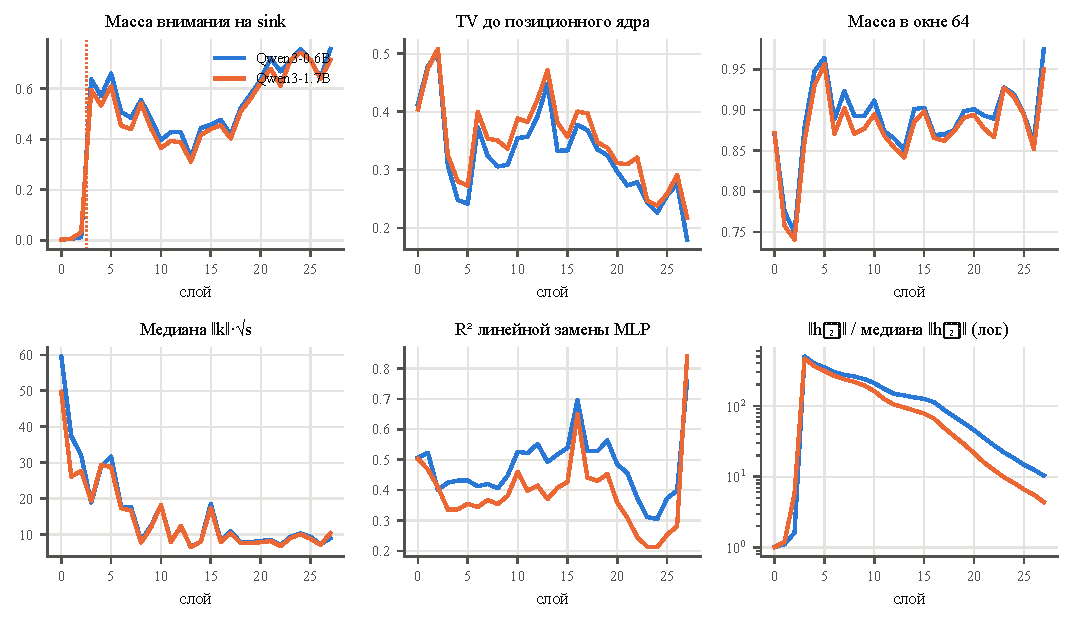
\includegraphics[width=\linewidth]{figures/profile.pdf}}
\caption{Послойный профиль Qwen3. Масса внимания на стоке (позиция 0);
расстояние полной вариации до позиционного ядра (меньше "--- позиционнее);
доля массы внимания в окне 64; медианная масштабированная норма ключей;
$R^2$ линейной замены MLP на отложенных данных; отношение нормы первого
токена к медиане остальных. Пунктир "--- $k_{\mathrm{sink}}$.}
\label{fig:profile}
\end{figure}

На Qwen3-0.6B первые три слоя образуют отдельный режим (рис.~\ref{fig:profile}).
В слоях 0--2 сток внимания практически отсутствует: доля массы на
позиции 0 составляет $0.3$--$1.3\%$ против $32$--$77\%$ в последующих
слоях. Норма состояния первого токена выросла с ${\approx}20$ до
${\approx}7000$ к моменту входа в слой~3. Поэтому $k_{\mathrm{sink}}=3$.
Вопреки исходной гипотезе о <<позиционных>> первых слоях, расстояние
до позиционного ядра в слоях 0--2 наибольшее
($\mathrm{TV}\approx0.42$--$0.50$ против $0.30$ в среднем по слоям 3--27,
разброс $0.17$--$0.44$): внимание
первых слоёв в основном контентное. Это мотивирует метод O4.
На Qwen3-1.7B картина та же: $k_{\mathrm{sink}}=3$, норма первого
токена достигает ${\approx}14\,700$ на входе слоя~3.

\subsection{Случайные признаки неприменимы к первым слоям}

\begin{figure}[t]
\centering
\figorpending{figures/favor.pdf}{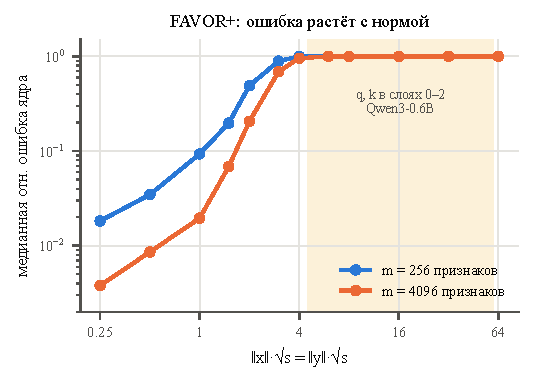
\includegraphics[width=0.55\linewidth]{figures/favor.pdf}}
\caption{Медианная относительная ошибка оценки $\exp(x^\top y)$
признаками FAVOR+ в зависимости от нормы входа ($D=128$, 64 пары на
точку, ошибка ограничена сверху единицей). Закрашенная
область "--- нормы запросов и ключей в слоях 0--2 Qwen3-0.6B.}
\label{fig:favor}
\end{figure}

Дисперсия оценки FAVOR+ растёт как $\exp(\|x+y\|^2)$. Для $m=4096$
признаков медианная относительная ошибка равна $2\%$ при
$\|x\|\sqrt s=\|y\|\sqrt s=1$, $21\%$ при $2$, $69\%$ при $3$ и
${\approx}100\%$ начиная с $4$. У Qwen3-0.6B после QK-нормализации медианная
масштабированная норма ключей в слоях 0--2 равна $32$--$60$, запросов
"--- $4.5$--$8$ (рис.~\ref{fig:favor}). Оценка ядра в этой области
бессмысленна, и замена внимания Performer без переобучения разрушает
модель. Мы проверили, что реализация несмещённая при малых нормах, то
есть это свойство модели, а не ошибка кода.

\subsection{Зависимость от глубины замены}

\begin{figure}[t]
\centering
\figorpending{figures/howmany.pdf}{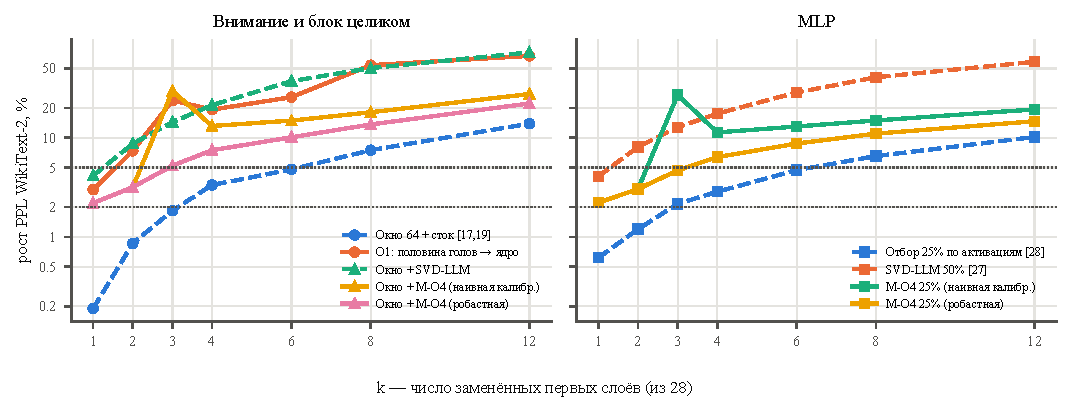
\includegraphics[width=\linewidth]{figures/howmany.pdf}}
\caption{Рост PPL WikiText-2 в зависимости от числа заменённых первых
слоёв $k$ (Qwen3-0.6B, 32 окна по 1024 токена, логарифмическая шкала;
пунктирные линии "--- пороги 2 и 5\,\%). Пунктир с кружками "--- методы из
литературы, сплошные с квадратами "--- предложенные; для M-O4 показаны
наивная и робастная калибровка (разд.~\ref{sec:propagation}).}
\label{fig:howmany}
\end{figure}

Окно со стоком деградирует плавно: 0.2, 0.9, 1.8, 3.3, 4.8, 7.5 и
13.9\,\% при $k = 1, 2, 3, 4, 6, 8, 12$, то есть первые три слоя
внимания заменяются в пределах 2\,\%, первые шесть "--- в пределах 5\,\%,
и даже при замене почти половины слоёв потеря остаётся умеренной. Отбор
25\,\% нейронов по готовым активациям ведёт себя похоже (0.6 "--- 10.2\,\%),
но экономит лишь последнюю матрицу MLP. SVD-LLM и O1 разваливаются
быстро: 12.8 и 23.7\,\% уже при $k=3$, более 50\,\% при $k=8$. Наивно
откалиброванный M-O4 демонстрирует немонотонность с пиком при
$k = k_{\mathrm{sink}} = 3$; её причина и устранение "--- в
разд.~\ref{sec:propagation}, после чего M-O4 удерживает 5\,\% до $k=3$ и
остаётся лучшим из методов с предсказанием нейронов до их вычисления.

\subsection{Качество и бюджет вычислений}

\begin{figure}[t]
\centering
\figorpending{figures/pareto.pdf}{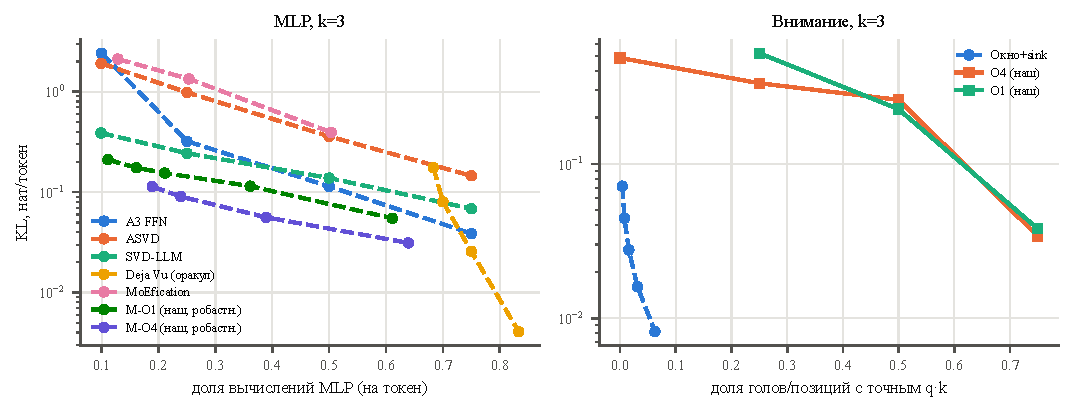
\includegraphics[width=\linewidth]{figures/pareto.pdf}}
\caption{KL в зависимости от бюджета при $k=k_{\mathrm{sink}}$ (Qwen3-0.6B).
Слева "--- методы для MLP (доля умножений на токен относительно
исходного MLP), справа "--- методы для внимания (доля вычисляемых
$q^\top k$).}
\label{fig:pareto}
\end{figure}

Ширина окна при $k=3$ задаёт плавный компромисс: 8, 16, 32, 64 и 128
позиций дают рост PPL 6.3, 4.1, 2.9, 1.8 и 1.0\,\%, то есть каждое
удвоение окна снимает около трети ошибки; 64 "--- колено кривой, которое мы
и используем. Для MLP отбор по вкладу нейрона при 5, 10, 25 и 50\,\%
активных даёт 16.9, 6.8, 2.2 и 0.3\,\%; робастный M-O4 с предсказанием
нейронов "--- 10.2, 7.8, 4.7 и 2.5\,\% при стоимости $0.28$--$0.55$ MLP;
SVD-LLM при ранге 10--75\,\% "--- от 41.5 до 5.8\,\%; A3 FFN "--- от $10^3$\,\%
при 10\,\% нейронов до 3.1\,\% при 75\,\%; ASVD и MoEfication уступают
всем. Для внимания половина голов, заменённых позиционным ядром (O1),
стоит 23.7\,\%, четверть "--- 2.9\,\%, три четверти "--- 67\,\%: позиционными
являются лишь немногие головы первых слоёв.

\subsection{Единый обменный курс}

\begin{figure}[t]
\centering
\figorpending{figures/exchange.pdf}{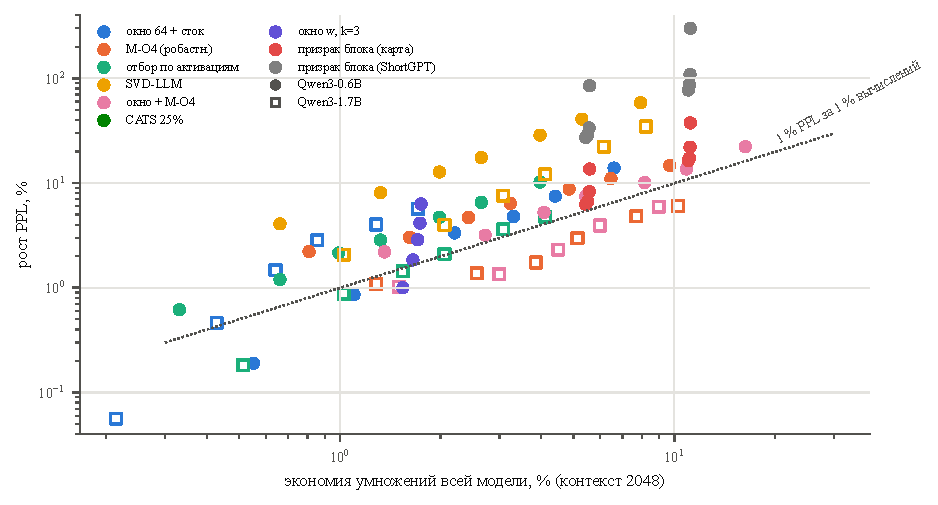
\includegraphics[width=0.9\linewidth]{figures/exchange.pdf}}
\caption{Все замены на одной шкале: рост PPL против доли сэкономленных
умножений всей модели при контексте 2048 (кривые по $k$, ширина окна,
призраки блоков; закрашенные маркеры "--- Qwen3-0.6B, пустые "--- 1.7B).
Пунктир "--- один процент PPL за один процент вычислений.}
\label{fig:exchange}
\end{figure}

На рис.~\ref{fig:exchange} все работающие детерминированные замены
Qwen3-0.6B ложатся около линии <<один процент PPL за один процент
вычислений>>: окно при $k=3$ (1.7\,\% экономии за 1.8\,\%), робастный M-O4
при $k=3$ ($\approx 4.6$ за 4.7\,\%), линейный призрак двух средних слоёв
(6.5 за 6.2\,\%). Методы с ошибочным критерием "--- SVD-LLM, CATS, призраки
по косинусному критерию ShortGPT "--- лежат в разы выше. У Qwen3-1.7B курс
лучше примерно в 2.5 раза: те же замены стоят 0.4\,\% PPL за процент
вычислений. Это основной аргумент в пользу проверки на моделях 4B--32B:
если курс продолжает улучшаться с размером, замена первых слоёв
становится выгодной именно там, где важна.

\subsection{Призраки блоков: где удалять слои}

Линейная замена блока из $n$ подряд идущих слоёв
(ReplaceMe~\cite{shopkhoev2025replaceme}) требует выбрать блок.
Критерий ShortGPT "--- косинусная близость входа и выхода слоя "--- на
Qwen3-0.6B выбирает слои 24--25 и 23--26; их удаление стоит $+85$ и
$+1760\,\%$ PPL, а линейная карта на границе снижает это лишь до 27 и
77\,\%. Выбор по нашей карте (минимальный KL одиночного удаления) даёт
слои 13--14 и 12--15: удаление $+13.6$ и $+37.5\,\%$, с полной линейной
картой $6.2$ и $16.4\,\%$, с картой ранга 256 "--- $6.7$ и $17.3\,\%$. Карта
заменяемости, построенная за один прогон одиночных замен, выбирает блок
в 4--5 раз точнее косинусного критерия, а призрак двух средних слоёв по
цене сопоставим с заменой MLP трёх первых.

\subsection{Итоговая таблица}

\begin{table}[t]
\centering
\scriptsize
\setlength{\tabcolsep}{3pt}
\IfFileExists{tables/final_0.6b.tex}{\begin{tabular}{lrrrrrrrrrrr}
\toprule
 & Исх. & Окно & Окно$_m$ & Поз. & A3 & SVD-LLM & Окно+SVD & O1 & M-O4 & M-O4r & Окно+M-O4r \\
\midrule
Что заменено & — & вним. & вним. & вним. & блок & MLP & блок & вним. & MLP & MLP & блок \\
Доля вычислений MLP & 1.00 & 1.00 & 1.00 & 1.00 & 0.50 & 0.50 & 0.50 & 1.00 & 0.39 & 0.39 & 0.39 \\
PPL WikiText-2 $\downarrow$ & 14.06 & 14.32 & 14.32 & 84.26 & 20.98 & 15.85 & 16.08 & 17.39 & 17.86 & 14.72 & 14.79 \\
KL к исходной $\downarrow$ & 0.000 & 0.016 & 0.016 & 1.805 & 0.433 & 0.138 & 0.151 & 0.226 & 0.268 & 0.056 & 0.065 \\
Совпадение top-1 $\uparrow$ & 100.0 & 94.7 & 94.7 & 43.4 & 71.6 & 85.4 & 84.3 & 80.3 & 76.1 & 90.5 & 89.4 \\
LAMBADA $\uparrow$ & 53.5 & 55.0 & 55.0 & 14.5 & 36.5 & 46.0 & 46.0 & — & 32.5 & 51.0 & 51.5 \\
HellaSwag $\uparrow$ & 53.0 & 53.5 & 53.5 & 47.0 & 47.5 & 53.0 & 53.0 & — & 48.5 & 54.0 & 53.0 \\
ARC-e $\uparrow$ & 55.5 & 57.5 & 57.5 & 49.5 & 54.0 & 61.0 & 61.0 & — & 57.0 & 58.0 & 57.0 \\
ARC-c $\uparrow$ & 36.0 & 37.0 & 37.0 & 28.5 & 30.0 & 35.0 & 35.0 & — & 31.0 & 37.0 & 38.0 \\
PIQA $\uparrow$ & 72.0 & 70.5 & 70.5 & 61.0 & 64.5 & 67.5 & 68.0 & — & 64.0 & 69.0 & 68.0 \\
WinoGrande $\uparrow$ & 63.0 & 63.0 & 63.0 & 58.0 & 57.0 & 59.0 & 59.5 & — & 53.5 & 64.5 & 65.5 \\
MMLU (5-shot) $\uparrow$ & 51.6 & 50.9 & 51.6 & 29.1 & 37.2 & 48.8 & 46.0 & — & 24.6 & 48.8 & 47.0 \\
Среднее по бенчам $\uparrow$ & 54.9 & 55.3 & 55.4 & 41.1 & 46.7 & 52.9 & 52.6 & — & 44.4 & 54.6 & 54.3 \\
\bottomrule
\end{tabular}
}{\textcolor{red}{[ожидает прогона]}}
\caption{Qwen3-0.6B-Base, замена первых $k_{\mathrm{sink}}$ слоёв.
Столбцы: исходная модель; методы из литературы (окно+сток, позиционное
внимание, A3, SVD-LLM, окно+SVD-LLM); предложенные (O1, M-O4 с наивной
и робастной калибровкой, окно+M-O4 робастный). Бенчмарки "--- точность,
\%, подвыборки по 200 примеров (MMLU "--- 5 на подзадачу).}
\label{tab:final06}
\end{table}

\begin{table}[t]
\centering
\scriptsize
\setlength{\tabcolsep}{3pt}
\IfFileExists{tables/final_1.7b.tex}{\begin{tabular}{lrrrrrrrrrrr}
\toprule
 & Исх. & Окно & Окно$_m$ & Поз. & A3 & SVD-LLM & Окно+SVD & O1 & M-O4 & M-O4r & Окно+M-O4r \\
\midrule
Что заменено & — & вним. & вним. & вним. & блок & MLP & блок & вним. & MLP & MLP & блок \\
Доля вычислений MLP & 1.00 & 1.00 & 1.00 & 1.00 & 0.50 & 0.50 & 0.50 & 1.00 & 0.38 & 0.38 & 0.38 \\
PPL WikiText-2 $\downarrow$ & 10.39 & 10.54 & 10.54 & 22.07 & 15.06 & 11.18 & 11.33 & 11.36 & 10.60 & 10.57 & 10.63 \\
KL к исходной $\downarrow$ & 0.000 & 0.019 & 0.019 & 0.781 & 0.408 & 0.091 & 0.104 & 0.088 & 0.031 & 0.028 & 0.037 \\
Совпадение top-1 $\uparrow$ & 100.0 & 94.3 & 94.4 & 62.5 & 73.9 & 88.8 & 87.5 & 87.9 & 93.5 & 94.0 & 92.4 \\
LAMBADA $\uparrow$ & 64.0 & 63.5 & 64.0 & 36.0 & 51.0 & 60.5 & 61.0 & 60.5 & 64.5 & 64.0 & 65.5 \\
HellaSwag $\uparrow$ & 57.0 & 59.5 & 59.5 & 55.0 & 55.5 & 58.0 & 57.5 & 57.5 & 56.5 & 59.5 & 60.0 \\
ARC-e $\uparrow$ & 68.0 & 69.0 & 69.0 & 69.5 & 59.5 & 71.5 & 72.0 & 74.0 & 70.5 & 70.5 & 72.0 \\
ARC-c $\uparrow$ & 43.5 & 43.5 & 43.5 & 43.0 & 38.0 & 47.0 & 46.5 & 45.5 & 46.0 & 43.5 & 44.5 \\
PIQA $\uparrow$ & 77.5 & 79.0 & 79.0 & 75.5 & 69.5 & 72.5 & 72.0 & 75.5 & 73.0 & 77.0 & 76.0 \\
WinoGrande $\uparrow$ & 61.5 & 61.0 & 61.0 & 56.0 & 55.5 & 62.5 & 63.0 & 60.0 & 65.0 & 64.0 & 65.0 \\
MMLU (5-shot) $\uparrow$ & 64.6 & 65.6 & 67.7 & 37.2 & 45.6 & 58.9 & 58.2 & 64.9 & 63.5 & 66.3 & 64.2 \\
Среднее по бенчам $\uparrow$ & 62.3 & 63.0 & 63.4 & 53.2 & 53.5 & 61.6 & 61.5 & 62.6 & 62.7 & 63.5 & 63.9 \\
\bottomrule
\end{tabular}
}{\textcolor{red}{[ожидает прогона]}}
\caption{Qwen3-1.7B-Base, те же столбцы, что в табл.~\ref{tab:final06}.}
\label{tab:final17}
\end{table}

\paragraph{Статистическая значимость.} На подвыборках по 200 примеров
стандартная ошибка средней точности по семи задачам равна $\pm2.5$ п.п.,
на 1000 примерах "--- $\pm1.1$ п.п. (биномиальная оценка). На 1000 примерах
окно при $k=3$ даёт 54.7 против 54.5\,\% у исходной Qwen3-0.6B и 62.9
против 62.4\,\% у 1.7B "--- неотличимо от исходной модели. Робастный M-O4
на 0.6B теряет около пункта (53.5\,\%, на границе значимости), на 1.7B
"--- нет (62.7\,\%); SVD-LLM теряет один--два пункта значимо (52.5 и
61.5\,\%). Для PPL и KL 95\,\%-е интервалы по бутстрэпу окон на полном
тесте WikiText-2 узки: окно 1.6 [1.5; 1.7]\,\%, робастный M-O4 4.9
[4.6; 5.1]\,\%, SVD-LLM 13.2 [12.6; 13.8]\,\% на 0.6B; 1.7 [1.6; 1.8], 1.7
[1.5; 1.9] и 8.2 [7.7; 8.7]\,\% на 1.7B (табл.~\ref{tab:ci}). Все
различия между главными столбцами значимы.

\begin{table}[t]
\centering
\scriptsize
\IfFileExists{tables/ci_0.6b.tex}{\begin{tabular}{lllll}
\toprule
Конфигурация & рост PPL, \% [95\% ДИ] & KL [95\% ДИ] & среднее по бенчам ± 1.96 SE & источник \\
\midrule
orig & 0.0 [0.0; 0.0] & 0.000 [0.000; 0.000] & 54.5 ± 1.1 & ci+bench1000 \\
L1-window64 & 1.6 [1.5; 1.7] & 0.015 [0.015; 0.015] & 54.7 ± 1.1 & ci+bench1000 \\
MO4-routed25r & 4.9 [4.6; 5.1] & 0.059 [0.057; 0.061] & 53.5 ± 1.1 & ci+bench1000 \\
ML5-svdllm50 & 13.2 [12.6; 13.8] & 0.145 [0.140; 0.151] & 52.5 ± 1.1 & ci+bench1000 \\
B-window+MO4-25r & 5.4 [5.1; 5.7] & 0.067 [0.065; 0.070] & 53.5 ± 1.1 & ci+bench1000 \\
\bottomrule
\end{tabular}
}{\textcolor{red}{[ожидает прогона]}}
\caption{Qwen3-0.6B, $k=3$: рост PPL и KL на полном тесте WikiText-2 с
95\,\%-ми интервалами по бутстрэпу окон (283 окна по 1024 токена).}
\label{tab:ci}
\end{table}

\subsection{Длина контекста и число стоков}

Ошибка окна растёт с длиной контекста медленно, примерно как логарифм
$T$: при $k=3$ она равна 1.81, 2.51, 3.21 и 4.89\,\% для $T = 1024$, 2048,
4096 и 8192 (табл.~\ref{tab:long}); четыре стока вместо одного помогают
лишь при $T=8192$ (4.49\,\%). Число стоков "--- один, два, четыре или сток
вместе со всеми токенами перевода строки "--- на результат не влияет
(разброс 0.03 п.п. при $k=3$ и $k=6$).

\begin{table}[t]
\centering
\small
\IfFileExists{tables/long.tex}{\begin{tabular}{lrrrr}
\toprule
Контекст $T$ & 1024 & 2048 & 4096 & 8192 \\
\midrule
$k=3$, 1 сток & 1.81\% & 2.51\% & 3.21\% & 4.89\% \\
$k=3$, 4 стока & 1.80\% & 2.48\% & 3.18\% & 4.49\% \\
\midrule
$k=3$, 2 стока & 1.81\% & 2.49\% & — & — \\
$k=3$, сток + переводы строки & 1.80\% & 2.49\% & — & — \\
$k=6$, 2 стока & 4.69\% & 6.27\% & — & — \\
$k=6$, сток + переводы строки & 4.71\% & 6.28\% & — & — \\
\bottomrule
\end{tabular}
}{\textcolor{red}{[ожидает прогона]}}
\caption{Окно 64 в первых $k$ слоях Qwen3-0.6B: рост PPL в зависимости
от длины контекста и числа стоков (бюджет 65 тыс. токенов на длину).}
\label{tab:long}
\end{table}

\subsection{Перенос на другой корпус}

\begin{figure}[t]
\centering
\figorpending{figures/domain.pdf}{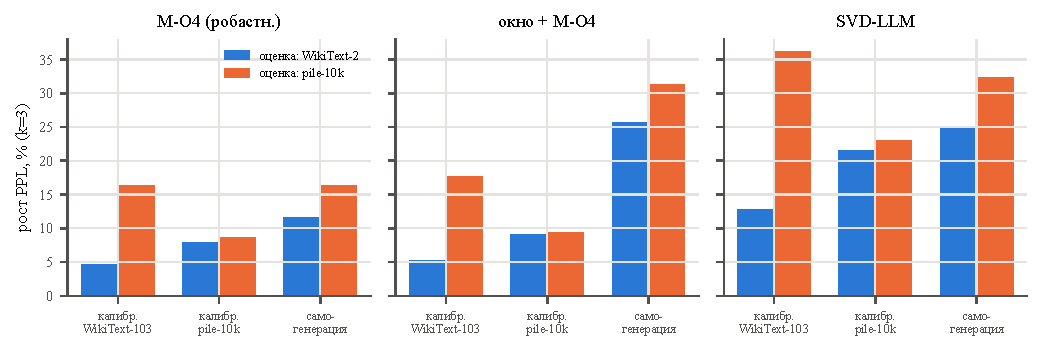
\includegraphics[width=\linewidth]{figures/domain.pdf}}
\caption{Домен калибровки (Qwen3-0.6B, $k=3$): рост PPL на WikiText-2 и
на pile-10k при калибровке на WikiText-103, на pile-10k и на тексте,
сгенерированном самой моделью.}
\label{fig:domain}
\end{figure}

Окно не калибруется и переносится без потерь: 1.2\,\% на pile-10k против
1.8\,\% на WikiText-2. Калиброванные замены MLP переобучаются под домен
калибровки: при калибровке на WikiText-103 робастный M-O4 стоит 4.7\,\% на
WikiText-2 и 16.4\,\% на pile-10k, SVD-LLM "--- 12.8 и 36\,\%
(рис.~\ref{fig:domain}). Калибровка на pile-10k выравнивает ошибку
(8.6 и 8.0\,\% у M-O4, 23 и 21.5\,\% у SVD-LLM), то есть смешанная
калибровка "--- рабочее лекарство; текст, сгенерированный самой моделью,
лекарством не является (16.3 и 11.6\,\%): сэмплы нерепрезентативны.

\subsection{Второе семейство: SmolLM2-1.7B и Llama-3.2-1B}
\label{sec:family2}

Таблицы~\ref{tab:finalsmol} и~\ref{tab:finalllama} повторяют итоговую
таблицу для двух моделей архитектуры Llama. Глубина $k_{\mathrm{sink}}$
определяется профилем автоматически: у Llama-3.2-1B массивная активация
позиции~0 (норма 794 при медиане 2.4) появляется после слоя~1, как у
Qwen3 "--- после слоя~2, поэтому $k_{\mathrm{sink}}=2$; у SmolLM2 сток
позиции~0 (норма $26\,235$) возникает лишь после слоя~7, $k_{\mathrm{sink}}=8$.
Три вывода. (1) Правило стока в исходном виде (<<позиция~0>>) для этого
семейства неверно: окно 64 с одним стоком даёт $+64\,\%$ PPL на SmolLM2
при $k=8$ и $+13\,\%$ на Llama-3.2-1B при $k=2$, тогда как то же окно с
правилом <<сток "--- массивный ключ>> (разд.~\ref{sec:tokensinks}) "---
$4.4$ и $2.8\,\%$, то есть столько же слоёв, сколько у Qwen3 при пороге
5\,\%. На кривой по $k$ у SmolLM2 окно с позиционным стоком стоит 0.7, 2.1,
13.7, 27.3, 62.4 и 64.1\,\% при $k=1,2,3,4,6,8$; с массивными стоками "---
0.8, 1.8, 2.0, 2.2, 3.5 и 4.4\,\% при тех же $k$, то есть та же форма кривой,
что у Qwen3. (2) MLP первых слоёв у
Llama-семейства заменяется заметно хуже, чем у Qwen3: робастный M-O4 стоит
$16\,\%$ на Llama-3.2-1B уже при $k=2$ и $6.3\,\%$ на SmolLM2 при $k=1$
(34\,\% при $k=8$), SVD-LLM "--- 47 и 49\,\%, A3 "--- 97 и 499\,\%,
позиционное внимание (relpos) и типизация голов O1 рушатся при $k\ge2$.
Диагностика обрыва показывает, что усиление ошибки по слоям $k-1..k+1$ у
SmolLM2 равно 0.9--1.1, то есть обрыва нет: дорог сам первый MLP, а не
его последствия для стока. Оракульный отбор 25\,\% нейронов одного слоя~0
даёт KL 0.0046 (меньше, чем у Qwen3-0.6B), так что узкое место "---
линейный предиктор нейронов при $I/d=4$, а не отбор как таковой.
(3) Робастная калибровка и защита нейронов стока нужны здесь ещё
сильнее: наивная комбинация окно\,+\,M-O4 даёт $+1\,100\,\%$ на
Llama-3.2-1B и $+612\,\%$ на SmolLM2 ($k=2$), робастная с защитой "---
31.8 и 13.9\,\%; наивный M-O4 на SmolLM2 при $k=2$ стоит 123\,\%, с защитой
нейронов стока "--- 11.3\,\%. Бенчмарки в таблицах посчитаны на тех же
подвыборках, что и для Qwen3.

\begin{table}[t]
\centering
\scriptsize
\setlength{\tabcolsep}{3pt}
\IfFileExists{tables/final_smol1.7b.tex}{\begin{tabular}{lrrrrrrrrrrr}
\toprule
 & Исх. & Окно & Окно$_m$ & Поз. & A3 & SVD-LLM & Окно+SVD & O1 & M-O4 & M-O4r & Окно+M-O4r \\
\midrule
Что заменено & — & вним. & вним. & вним. & блок & MLP & блок & вним. & MLP & MLP & блок \\
Доля вычислений MLP & 1.00 & 1.00 & 1.00 & — & 0.50 & — & — & — & 0.35 & 0.35 & 0.35 \\
PPL WikiText-2 $\downarrow$ & 8.93 & 14.65 & 9.32 & — & 53.47 & — & — & — & 12.00 & 12.00 & 17.74 \\
KL к исходной $\downarrow$ & 0.000 & 0.503 & 0.044 & — & 1.795 & — & — & — & 0.314 & 0.313 & 0.713 \\
Совпадение top-1 $\uparrow$ & 100.0 & 79.3 & 91.2 & — & 48.4 & — & — & — & 77.6 & 77.7 & 65.7 \\
LAMBADA $\uparrow$ & 71.0 & 66.5 & 71.5 & — & 27.5 & — & — & — & 34.0 & 35.0 & 16.5 \\
HellaSwag $\uparrow$ & 64.0 & 63.5 & 63.5 & — & 41.0 & — & — & — & 52.5 & 52.0 & 46.0 \\
ARC-e $\uparrow$ & 75.0 & 75.5 & 75.5 & — & 32.5 & — & — & — & 57.5 & 56.0 & 43.0 \\
ARC-c $\uparrow$ & 43.0 & 43.5 & 43.5 & — & 19.0 & — & — & — & 29.0 & 30.0 & 25.0 \\
PIQA $\uparrow$ & 78.0 & 78.0 & 78.5 & — & 51.0 & — & — & — & 62.0 & 63.0 & 58.5 \\
WinoGrande $\uparrow$ & 65.0 & 66.0 & 66.0 & — & 46.5 & — & — & — & 58.0 & 59.5 & 57.0 \\
MMLU (5-shot) $\uparrow$ & 56.1 & 54.0 & 53.0 & — & 22.5 & — & — & — & 28.1 & 29.5 & 21.4 \\
Среднее по бенчам $\uparrow$ & 64.6 & 63.9 & 64.5 & — & 34.3 & — & — & — & 45.9 & 46.4 & 38.2 \\
\bottomrule
\end{tabular}
}{\textcolor{red}{[ожидает прогона]}}
\caption{SmolLM2-1.7B, замена первых $k_{\mathrm{sink}}=8$ слоёв; столбцы
как в табл.~\ref{tab:final06} (конфигурации, не поместившиеся в память
ноутбука при $k=8$, опущены). Окно с массивными стоками (L1-window64s) "---
правило разд.~\ref{sec:tokensinks}.}
\label{tab:finalsmol}
\end{table}

\begin{table}[t]
\centering
\scriptsize
\setlength{\tabcolsep}{3pt}
\IfFileExists{tables/final_llama1b.tex}{\begin{tabular}{lrrrrrrrrrrr}
\toprule
 & Исх. & Окно & Окно$_m$ & Поз. & A3 & SVD-LLM & Окно+SVD & O1 & M-O4 & M-O4r & Окно+M-O4r \\
\midrule
Что заменено & — & вним. & вним. & вним. & блок & MLP & блок & вним. & MLP & MLP & блок \\
Доля вычислений MLP & 1.00 & 1.00 & 1.00 & 1.00 & 0.50 & 0.50 & 0.50 & 1.00 & 0.35 & 0.35 & 0.35 \\
PPL WikiText-2 $\downarrow$ & 11.31 & 12.80 & 11.62 & 8803.33 & 22.23 & 16.58 & 20.87 & 14.75 & 13.14 & 13.14 & 14.90 \\
KL к исходной $\downarrow$ & 0.000 & 0.113 & 0.030 & 6.630 & 0.665 & 0.384 & 0.602 & 0.258 & 0.151 & 0.152 & 0.280 \\
Совпадение top-1 $\uparrow$ & 100.0 & 86.2 & 92.5 & 1.0 & 65.4 & 74.1 & 67.8 & 78.5 & 84.2 & 84.1 & 77.9 \\
LAMBADA $\uparrow$ & 59.0 & 59.0 & 59.0 & 0.0 & 44.5 & 45.0 & 45.5 & 59.5 & 55.5 & 54.0 & 50.5 \\
HellaSwag $\uparrow$ & 58.0 & 59.0 & 59.0 & 31.5 & 55.5 & 57.5 & 57.5 & 57.5 & 57.0 & 55.5 & 54.5 \\
ARC-e $\uparrow$ & 60.5 & 61.0 & 61.0 & 26.0 & 50.0 & 52.5 & 53.0 & 61.0 & 58.5 & 58.0 & 55.5 \\
ARC-c $\uparrow$ & 32.5 & 32.5 & 32.5 & 27.0 & 27.5 & 28.5 & 28.0 & 33.5 & 32.5 & 32.0 & 34.0 \\
PIQA $\uparrow$ & 76.5 & 75.5 & 75.5 & 46.5 & 67.0 & 71.5 & 72.5 & 75.5 & 70.0 & 70.0 & 69.0 \\
WinoGrande $\uparrow$ & 62.5 & 63.5 & 63.5 & 51.0 & 54.5 & 58.0 & 57.0 & 59.0 & 63.5 & 59.5 & 59.0 \\
MMLU (5-shot) $\uparrow$ & 35.1 & 32.6 & 32.6 & 27.0 & 26.3 & 26.0 & 28.8 & 28.8 & 32.3 & 29.1 & 28.8 \\
Среднее по бенчам $\uparrow$ & 54.9 & 54.7 & 54.7 & 29.9 & 46.5 & 48.4 & 48.9 & 53.5 & 52.8 & 51.2 & 50.2 \\
\bottomrule
\end{tabular}
}{\textcolor{red}{[ожидает прогона]}}
\caption{Llama-3.2-1B, замена первых $k_{\mathrm{sink}}=2$ слоёв; столбцы
как в табл.~\ref{tab:final06}.}
\label{tab:finalllama}
\end{table}

\subsection{Время}

\begin{table}[t]
\centering
\scriptsize
\setlength{\tabcolsep}{4pt}
\IfFileExists{tables/timing.tex}{\begin{tabular}{lrrrrrr}
\toprule
Модель & $T$ & \multicolumn{2}{c}{слой внимания, мс} & \multicolumn{2}{c}{prefill модели, мс} & отношение \\
 & & полное (SDPA) & лента (PyTorch) & исходная & первые 3 слоя --- лента & \\
\midrule
Qwen3-0.6B & 1024 & 2.3 & 99.1 & 950 & 1275 & 0.74 \\
Qwen3-0.6B & 2048 & 8.5 & 209.3 & 2009 & 2657 & 0.76 \\
Qwen3-0.6B & 4096 & 37.6 & 457.7 & 4547 & 5695 & 0.80 \\
Qwen3-0.6B & 8192 & 163.2 & 894.5 & 11058 & 13331 & 0.83 \\
Qwen3-1.7B & 1024 & 2.2 & 96.9 & 2205 & 2557 & 0.86 \\
Qwen3-1.7B & 2048 & 7.6 & 193.6 & 4691 & 5287 & 0.89 \\
Qwen3-1.7B & 4096 & 29.7 & 386.7 & 9550 & 10696 & 0.89 \\
Qwen3-1.7B & 8192 & 155.7 & 808.6 & 21185 & 23572 & 0.90 \\
\bottomrule
\end{tabular}
}{\textcolor{red}{[ожидает прогона]}}
\caption{Замер времени на Apple M4 (MPS, bf16, медиана 5 запусков):
ленточная реализация окна на чистом PyTorch против fused-ядра SDPA.}
\label{tab:timing}
\end{table}

Наша ленточная реализация окна на чистом PyTorch, хотя и имеет
асимптотику $O(Tw)$ и память $O(Tw)$, на MPS медленнее fused-ядра
полного внимания в 5--40 раз на уровне слоя и замедляет prefill модели
на 10--25\,\% (табл.~\ref{tab:timing}). Реальное ускорение возможно только
со специализированным ядром скользящего окна, которые существуют для
CUDA; все оценки экономии в работе "--- по числу умножений.
